\documentclass[accentcolor=tud8b,colorbacktitle]{tudbeamer}

\usepackage[utf8]{inputenc}
\usepackage{graphicx}
\usepackage{multicol}
\usepackage[most]{tcolorbox}
\usepackage{wasysym}

\title{\textcolor{white}{Collide, Collate, Collect:\\Decoding wireless collisions\\}}
\subtitle{\textcolor{white}{B.Sc. Thesis Progress\\Johannes Lauinger}}
\author{SEEMOO | Bachelor thesis progress | Johannes Lauinger}
\logo{
\includegraphics{../../gfx/logos/seemoo-logo}}
\date{22.05.2017}


\begin{document}

\begin{titleframe}
	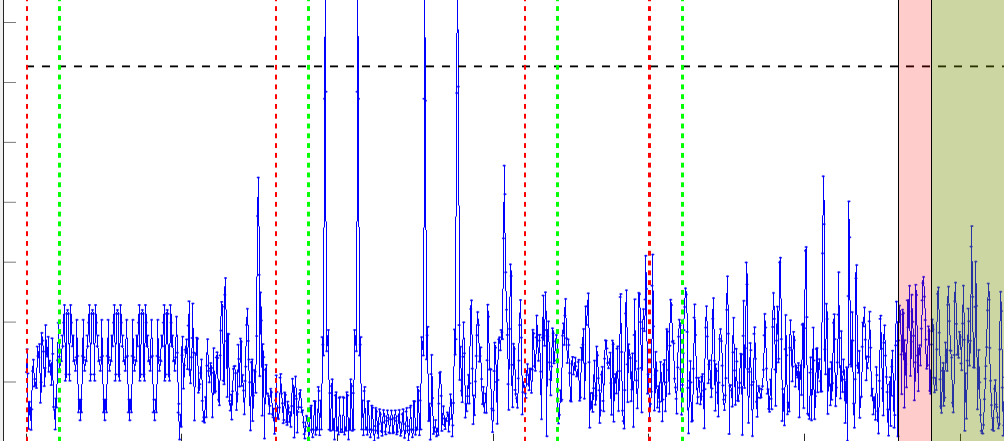
\includegraphics[width=12.1cm]{assets/title-image}
\end{titleframe}


\begin{frame}
\frametitle{Motivation}
\begin{itemize}
	\setlength\itemsep{1em}
	\item Collisions exist in IEEE 802.11 networks despite counter-measures
	\item Easy to spot a collision
	\item Hard to detect \textbf{which senders} collided
	\item Useful for new coordination functions
	\item A and B collide $\rightarrow$ C is next up for sending
	\item Also: statistics, network monitoring
\end{itemize}
\end{frame}


\begin{frame}
\frametitle{IEEE 802.11 Background: MAC}
\begin{center}
	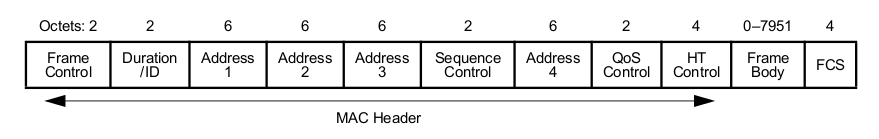
\includegraphics[width=12.1cm]{assets/mac-format}\\
	\small Figure: \cite{ieee2012} \normalsize\\~\\
	But: no Address 4, no QoS Control, no HT Control
\end{center}
\end{frame}


\begin{frame}
\frametitle{IEEE 802.11 Background: Frame Generation}
\begin{itemize}
	\item PSDU bit stream
	\item Prepend service bits, append tail and pad bits
	\item \textbf{Apply scrambler} (7 bit LFSR)
	\item \textbf{Apply convolutional encoding}
	\item Group into symbols, apply interleaving
	\item Modulate
	\item Insert Pilots
	\item \textbf{IFFT}
	\item Prepend Cyclic Prefix
	\item ...
\end{itemize}
\end{frame}


\begin{frame}
\frametitle{IEEE 802.11 Background: PHY}
\begin{center}
	\vspace{-0.3cm}
	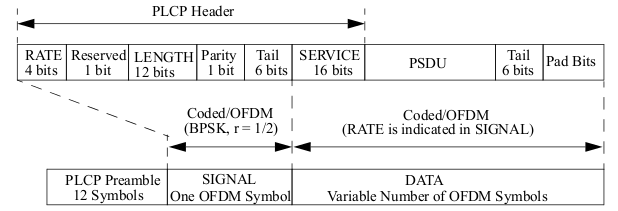
\includegraphics[width=8.1cm]{assets/phy-format}\\
	\vspace{0.2cm}
	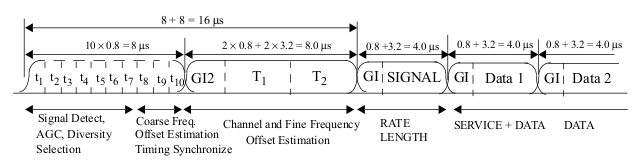
\includegraphics[width=11.1cm]{assets/preamble-format}\\
	\small Figures: \cite{ieee2012}
\end{center}
\end{frame}


\begin{frame}
\frametitle{Mathematical Background}
\begin{center}
Cross-correlation for discrete functions:
$$ (f \star g)(n) = \sum_{m=-\infty}^{\infty} f^{\ast}(m) g(m+n) $$\\
\vspace{0.5cm}
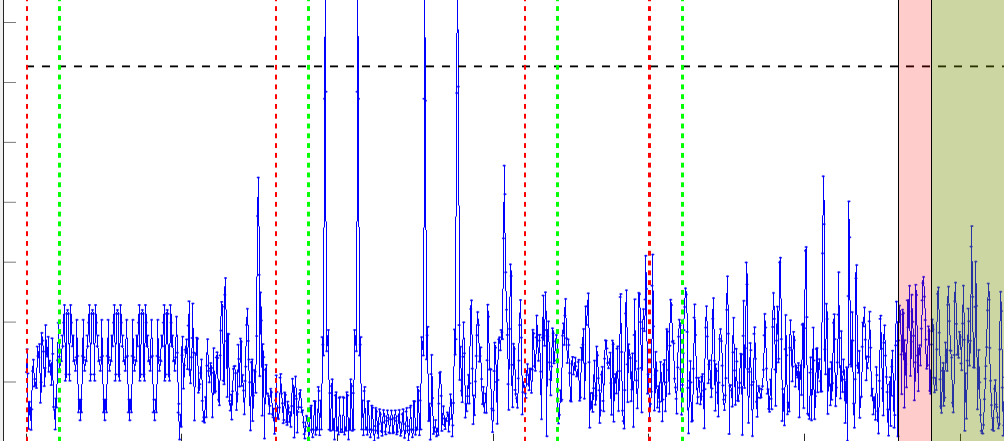
\includegraphics[width=8.1cm]{assets/title-image}
\end{center}
\end{frame}


\begin{frame}
\frametitle{Current Progress}
\begin{itemize}
	\setlength\itemsep{1em}
	\item Detect start of multiple packets in collision
	\item Try and correlate in frequency-domain (did not work)
	\item Simulate correlation in time-domain
	\item Quantize effects of varying different fields:
	\begin{itemize}
		\setlength\itemsep{1em}
		\item Scrambler initialization (essential)
		\item MSDU duration field / Destination Address (quite unimportant)
		\item Higher MCS
	\end{itemize}
\end{itemize}
\end{frame}


\begin{frame}
\frametitle{Current Progress - cont'd}
\begin{center}
	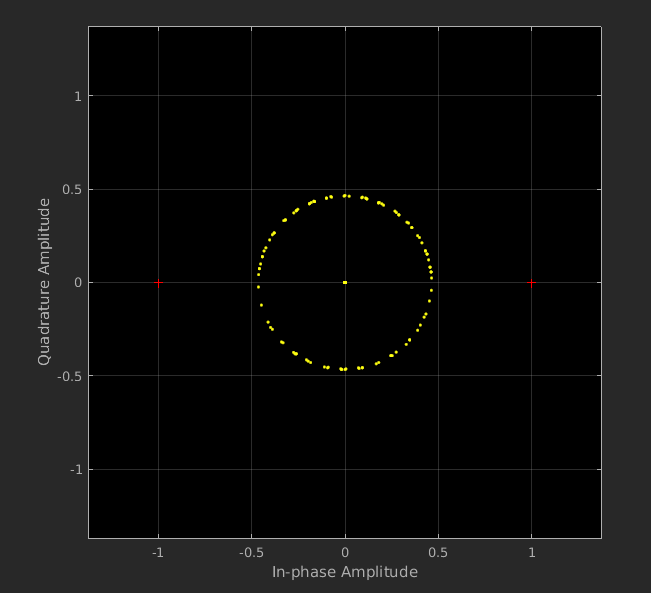
\includegraphics[height=6cm]{assets/freq-correlation}
\end{center}
\end{frame}


\begin{frame}
\frametitle{Current Progress - cont'd}
\begin{center}
	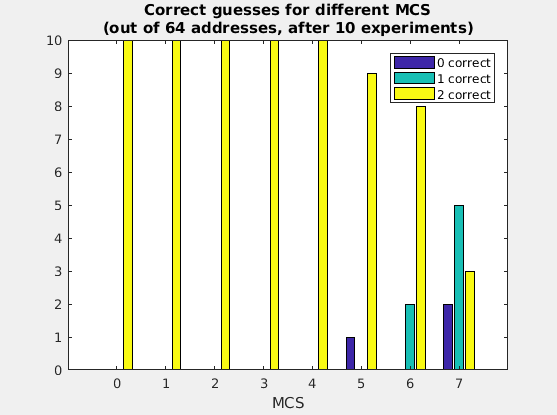
\includegraphics[height=6cm]{assets/higher-mcs}
\end{center}
\end{frame}


\begin{frame}
\frametitle{Timing and Complexity}
\textbf{Correlation at scale?}
\begin{itemize}
	\item xcorr for one frame under test: approx. 1ms
	\item Complexity: $O(\#MACs \cdot 127 \cdot 8) = O(n)$
	\item $O(n)$ for finding the best correlation
	\item However: approx. 300ms for generating one waveform
\end{itemize}
\vspace{0.5cm}
\textbf{Optimizations}
\begin{itemize}
	\item 1 Byte Frame Body
	\item Dummy FCS (0x00 00 00 00)
	\item Only correlate samples containing MAC address parts
	\item Pre-modulate pool of MAC addresses
\end{itemize}
\end{frame}


\begin{frame}
\frametitle{Real World Data Traits}
\begin{itemize}
	\setlength\itemsep{1em}
	\item Surprisingly diverse MAC address vendor bytes
	\item Scrambler initialization predictable to some extent \cite{noubir2016}
\end{itemize}
\end{frame}


\begin{frame}
\frametitle{Planned Work}
\begin{itemize}
	\setlength\itemsep{1em}
	\item Redo simulations with more data (ISP VM)
	\item Quantize AWGN, 802.11g stdchan, and TGn Channels
	\item Collect real frame collisions with WARP hardware
	\item Write thesis document \smiley
\end{itemize}
\end{frame}


\begin{frame}
\frametitle{Thank you for your attention!}
\begin{center}
	\huge Questions and discussion\\
	\vspace{0,6cm}
	
\includegraphics[height=4cm]{assets/faq}
\end{center}
\end{frame}


\begin{frame}[allowframebreaks]
\frametitle{References}
\bibliographystyle{plain}
\bibliography{../../config/bibliography}
\end{frame}

\end{document}
